% !TeX spellcheck = en_GB
A standard approach to model open quantum systems is the collision model.
The system under consideration interacts with a series of ancilla systems through a unitary transformation on the combined system-ancilla state \cite{Lorenzo_2017}. After a short interaction time $\Delta t$, the ancilla systems are traced out to obtain the system state.
We use this approach to model our setting, which consists of three qubits: the drive ($\ket{\psi_D}$), system and transducer ($\ket{\psi_T}$) qubits, where drive and transducer are considered ancilla qubits.
In general, a collision model approach leads to entanglement between system and ancilla.
This is undesirable in our model as we assume the drive and transducer to be in definitive, i.e. pure, states.
To ensure the ancilla and system states remain pure, we follow the approach used in \cite{beyer2020}:
let $\rho_S$ be the density operator of the system under consideration and $\ket{\psi_A} = \ket{\psi_D} \otimes \ket{\psi_T}$ the state of the ancilla system.
Given $\Delta t \ll 1$ the time evolution of $\rho_S$ under $H_{AS}$ acting on the 3 qubit Hilbert space is
\begin{align}\label{coll_eq}
\rho'_S & = \mathrm{Tr}_A \{ e^{-i H_{AS} \Delta t} (\ket{\psi_A} \bra{\psi_A} \otimes \rho_S) e^{i H_{AS} \Delta t} \} & = \rho_S - i \Delta t [\expval{H_{AS}}{\psi_A}, \rho_S] + O(\Delta t^2).
\end{align}

In the continuous limit Eq. (\ref{coll_eq}) leads to von-Neumann dynamics on the system for an infinite stream of qubits initialised in the same state $\ket{\psi_A}$:
\begin{align*}
	\dot{\rho}_S = - i [\expval{H_{AS}}{\psi_A}, \rho_S].
\end{align*}

As each ancilla only interacts once with the system and is traced out afterwards, $\rho_S$ remains pure in the limit of $\Delta t \to 0$.

We focus on piece-wise constant (PWC) functions of the drive ($\ket{\psi_D}$) and transducer ($\ket{\psi_T}$) qubits, as it greatly reduces computational complexity.
These are implemented by keeping the stream of ancillas $\ket{\psi_A} = \ket{\psi_D} \otimes \ket{\psi_T}$ constant for time $\Delta \mathrm{T}$ (Figure \ref{collmodel}).

\begin{figure}[h]
	\centering
	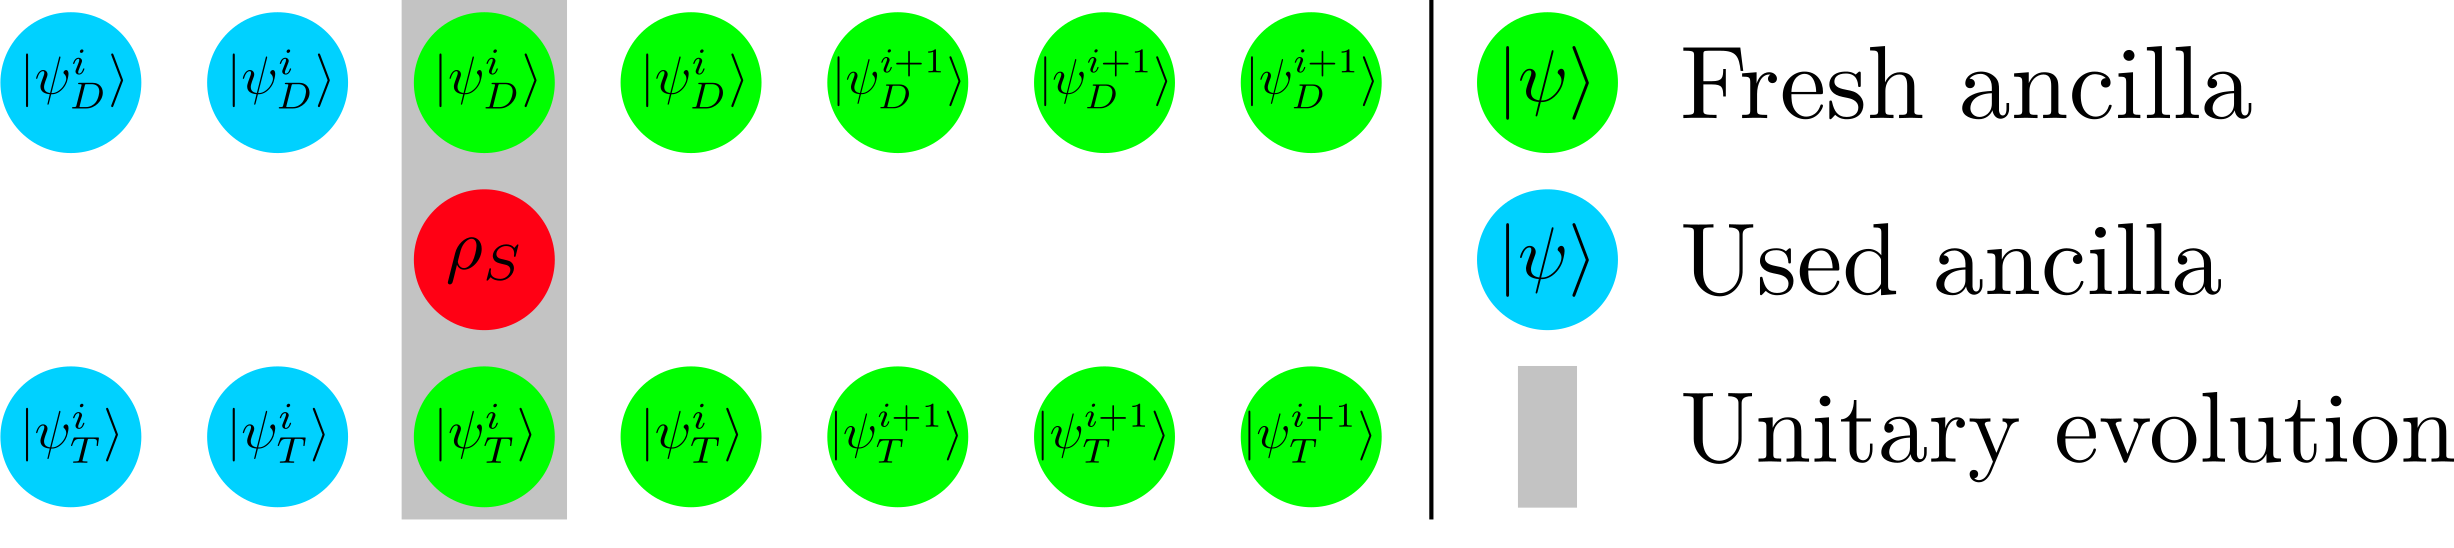
\includegraphics[width=0.85\textwidth]{img/coll2}
	\caption{Collision model used in this work: drive and transducer are series of qubits that interact once with the system and evolve the reduced density operator $\rho_S$. The qubit configuration can be changed in intervals of $\Delta \mathrm{T}$.}
	\label{collmodel}
\end{figure}

The drive and transducer qubits can be set in N discrete intervals represented by ($\theta_D^n, \phi_D^n$) and ($\theta_T^n, \phi_T^n$) respectively (see Figure \ref{pwc}), the system qubit is initialised in a pure state $\rho_S$.

\begin{figure}[h]
	\centering
	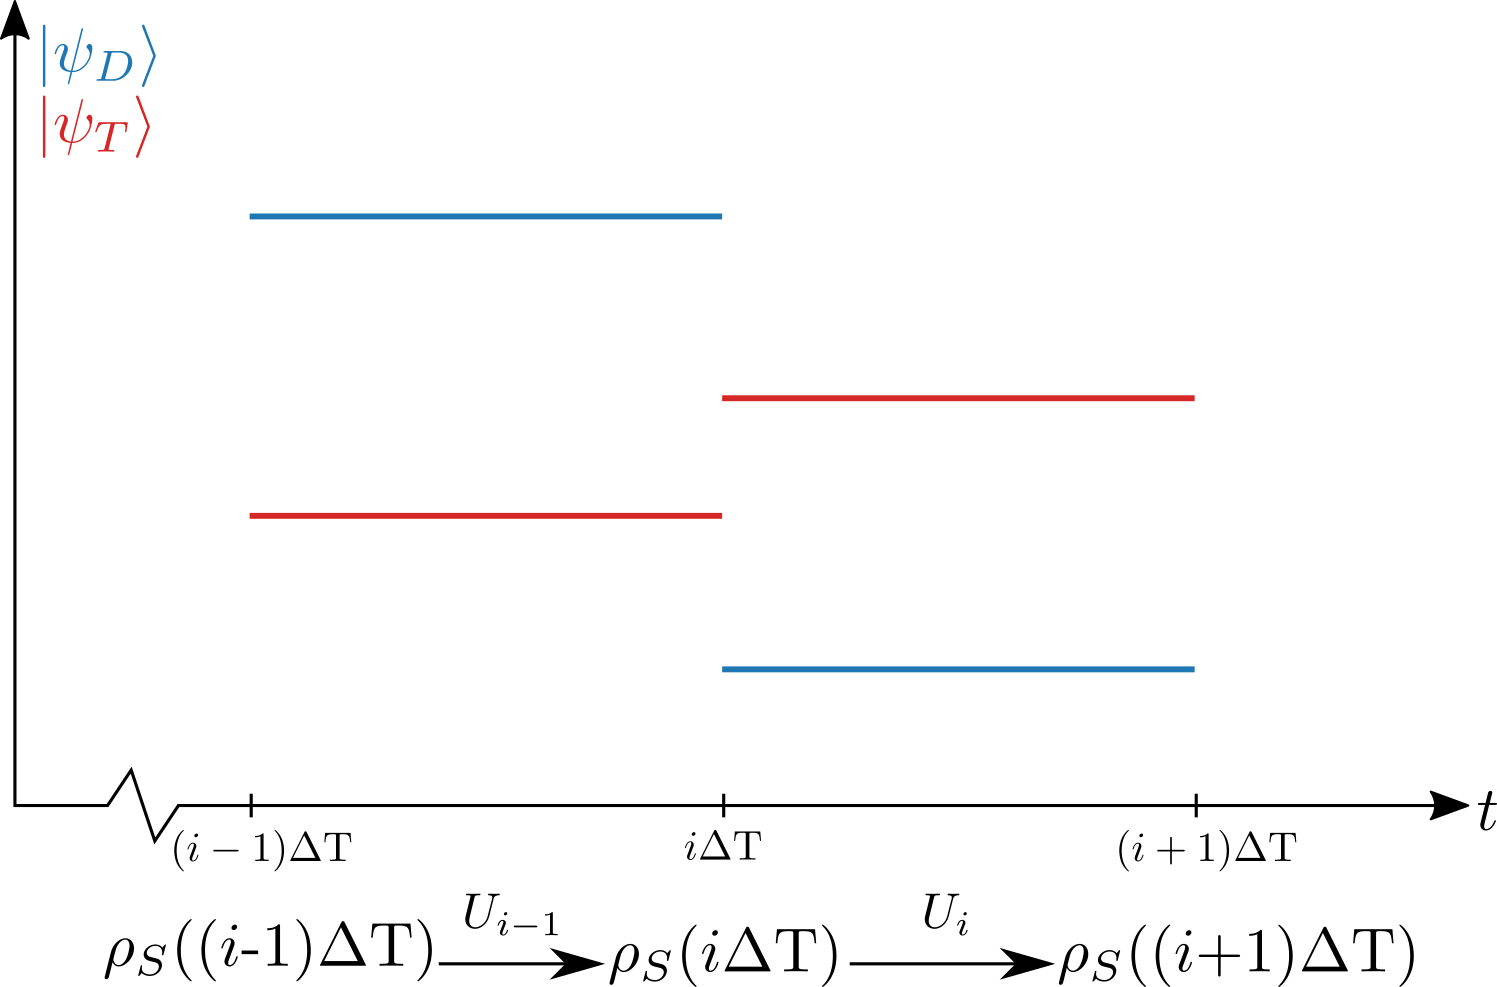
\includegraphics[width=0.6\textwidth]{img/pwc2}
	\caption{Piecewise constant implementation of drive and transducer qubits: the vertical axis represents an arbitrary parameter of the ancilla states. The qubit states are switched instantaneously and then kept constant for $\Delta \mathrm{T}$ while $\rho_S$ evolves unitarily. The piece-wise constant drive and transducer settings lead to a piece-wise constant system Hamiltonian.}
	\label{pwc}
\end{figure}

In the remainder of this work we use the interaction Hamiltonian on the three qubit Hilbert space
\begin{equation*}
H_{DST} = H^{I}_{DS} \otimes \mathds{1}_T + \mathds{1}_D \otimes H^{I}_{ST}, \\
H^{I} = \sigma_{+} \otimes \sigma_{-} + \sigma_{-} \otimes \sigma_{+}.
\end{equation*}
The Hamiltonians are unitless and therefore the interaction strength is given by the evolution time.
Note that the interaction Hamiltonian itself is constant and the time dependence comes from the change in the stream of ancillas only.
The energy scale of the Hamiltonian is therefore limited and so are the dynamics of the system state $\rho_S$.
The time evolution and work extraction is then calculated as follows, where $\Delta \mathrm{T}$ is the time span between qubit switching:
\begin{align}
H_S^n &= \bra{\psi_D^n}\bra{\psi_T^n} H_{DST} \ket{\psi_D^n} \ket{\psi_T^n}, \label{relham}\\
\rho_S &((n+1) \Delta \mathrm{T}) = U_n \ \rho_S(n \Delta \mathrm{T}) \ U^{\dagger}_n, \nonumber \\
U_n &= e^{-iH_S^n \Delta \mathrm{T}}, \nonumber \\ 
W &= \Sigma_n dW_n = - \Sigma_n \Tr{\rho_S(n \Delta \mathrm{T}) \ \Delta H_S^n}, \label{dw} \\
\Delta H_S^n &= \bra{\psi_D^n}\bra{\psi_T^{n+1}} H_{DST} \ket{\psi_D^n} \ket{\psi_T^{n+1}} - \bra{\psi_D^n}\bra{\psi_T^n} H_{DST} \ket{\psi_D^n} \ket{\psi_T^n}. \label{deltaham}
\end{align}
Here we use the partial Hamiltonian $H_S^n$ on the system at time step $n \in [1, N - 1]$, as well as the corresponding system density matrix $\rho_S(n \Delta \mathrm{T})$.
An advantage of this framework is that the extracted work is available to the experimenter as a quantum observable \cite{beyer2020}.

Using the Bloch sphere representation $\ket{\psi} = \cos(\frac{\theta}{2}) \ket{0} + e^{i \phi} \sin(\frac{\theta}{2})\ket{1}$ to represent drive and transducer qubits reduces Eq. (\ref{relham}) to
\begin{align}
H_S^n &= \frac{1}{2} \left[\sin(\theta_D^n) e^{i\phi_D^n} + \sin(\theta_T^n) e^{i\phi_T^n}\right] \sigma_{+} + h.c. =  H_{DS}^n + H_{ST}^n. \nonumber
\end{align}
In the following, we will call $H_{DS}$ the drive and $H_{ST}$ the transducer Hamiltonian, but note that both Hamiltonians act on the system Hilbert space only.
Eq. (\ref{deltaham}) can then be expressed in a simpler form
\begin{align}
\Delta H_S^n &= H_{ST}^{n+1} - H_{ST}^n. \label{simpledeltaham}
\end{align}